\documentclass[border=12pt]{standalone}
\usepackage{tikz,amsmath}
\usepackage[scaled]{helvet}
\renewcommand{\familydefault}{\sfdefault}
\usetikzlibrary{arrows.meta,positioning,calc,decorations.pathreplacing,patterns}
\definecolor{pro}{HTML}{1F5FA8}\definecolor{limb}{HTML}{C2410C}\definecolor{hot}{HTML}{DC2626}
\definecolor{good}{HTML}{15803D}\definecolor{ink}{HTML}{1F2937}\definecolor{quiet}{HTML}{6B7280}
\tikzset{>=Stealth,every node/.style={text=ink}}

\begin{document}
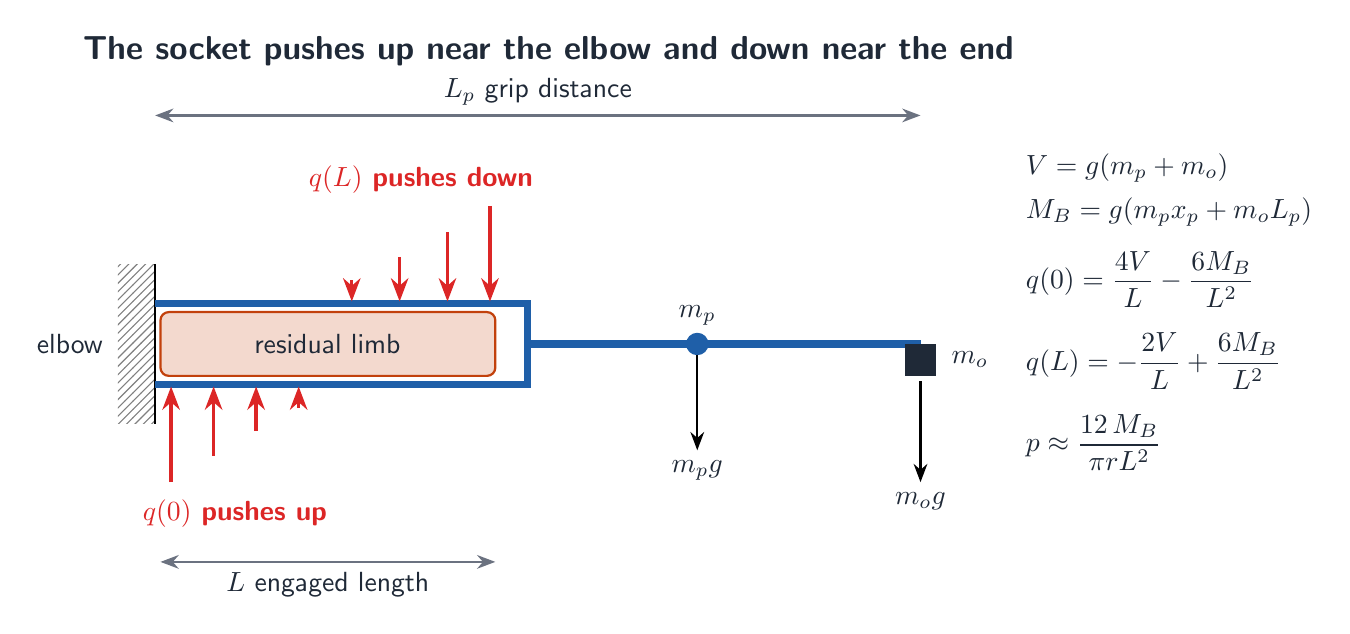
\begin{tikzpicture}[scale=1.35]
\node[font=\large\bfseries] at (3.7,2.75) {The socket pushes up near the elbow and down near the end};
\fill[pattern=north east lines,pattern color=gray] (-0.35,-0.75) rectangle (0,0.75); \draw[thick] (0,-0.75)--(0,0.75);
\node[left] at (-0.4,0) {elbow};
\fill[limb!20,draw=limb,thick,rounded corners=3pt] (0.05,-0.3) rectangle (3.2,0.3); \node at (1.62,0) {residual limb};
\draw[pro,line width=2.4pt] (0,0.38)--(3.5,0.38)--(3.5,-0.38)--(0,-0.38);
\draw[pro,line width=3pt] (3.5,0)--(7.2,0);
\fill[pro] (5.1,0) circle (3pt); \node[above] at (5.1,0.08) {$m_p$};
\draw[->,thick] (5.1,-0.1)--(5.1,-1.0) node[below] {$m_p g$};
\fill[ink] (7.05,-0.3) rectangle (7.35,0); \node[right] at (7.4,-0.15) {$m_o$};
\draw[->,thick] (7.2,-0.35)--(7.2,-1.3) node[below] {$m_o g$};
\foreach \x/\h in {0.15/0.9,0.55/0.65,0.95/0.42,1.35/0.2} \draw[->,hot,very thick] (\x,-0.4-\h)--(\x,-0.4);
\foreach \x/\h in {1.85/0.2,2.3/0.42,2.75/0.65,3.15/0.9} \draw[->,hot,very thick] (\x,0.4+\h)--(\x,0.4);
\node[hot,font=\bfseries] at (0.75,-1.6) {$q(0)$ pushes up};
\node[hot,font=\bfseries] at (2.5,1.55) {$q(L)$ pushes down};
\draw[<->,thick,quiet] (0.05,-2.05)--(3.2,-2.05) node[midway,below] {$L$ engaged length};
\draw[<->,thick,quiet] (0,2.15)--(7.2,2.15) node[midway,above] {$L_p$ grip distance};
\node[align=left,anchor=west] at (8.1,0.3) {$V=g(m_p+m_o)$\\[4pt]$M_B=g(m_px_p+m_oL_p)$\\[8pt]$q(0)=\dfrac{4V}{L}-\dfrac{6M_B}{L^2}$\\[8pt]$q(L)=-\dfrac{2V}{L}+\dfrac{6M_B}{L^2}$\\[8pt]$p\approx\dfrac{12\,M_B}{\pi rL^2}$};
\end{tikzpicture}
\end{document}
